
% Default to the notebook output style

    


% Inherit from the specified cell style.




    
\documentclass{article}

    
    
    \usepackage{graphicx} % Used to insert images
    \usepackage{adjustbox} % Used to constrain images to a maximum size 
    \usepackage{color} % Allow colors to be defined
    \usepackage{enumerate} % Needed for markdown enumerations to work
    \usepackage{geometry} % Used to adjust the document margins
    \usepackage{amsmath} % Equations
    \usepackage{amssymb} % Equations
    \usepackage[mathletters]{ucs} % Extended unicode (utf-8) support
    \usepackage[utf8x]{inputenc} % Allow utf-8 characters in the tex document
    \usepackage{fancyvrb} % verbatim replacement that allows latex
    \usepackage{grffile} % extends the file name processing of package graphics 
                         % to support a larger range 
    % The hyperref package gives us a pdf with properly built
    % internal navigation ('pdf bookmarks' for the table of contents,
    % internal cross-reference links, web links for URLs, etc.)
    \usepackage{hyperref}
    \usepackage{longtable} % longtable support required by pandoc >1.10
    \usepackage{booktabs}  % table support for pandoc > 1.12.2
    \usepackage{mathpazo}
    \usepackage[spanish]{babel}

    
    
    \definecolor{orange}{cmyk}{0,0.4,0.8,0.2}
    \definecolor{darkorange}{rgb}{.71,0.21,0.01}
    \definecolor{darkgreen}{rgb}{.12,.54,.11}
    \definecolor{myteal}{rgb}{.26, .44, .56}
    \definecolor{gray}{gray}{0.45}
    \definecolor{lightgray}{gray}{.95}
    \definecolor{mediumgray}{gray}{.8}
    \definecolor{inputbackground}{rgb}{.95, .95, .85}
    \definecolor{outputbackground}{rgb}{.95, .95, .95}
    \definecolor{traceback}{rgb}{1, .95, .95}
    % ansi colors
    \definecolor{red}{rgb}{.6,0,0}
    \definecolor{green}{rgb}{0,.65,0}
    \definecolor{brown}{rgb}{0.6,0.6,0}
    \definecolor{blue}{rgb}{0,.145,.698}
    \definecolor{purple}{rgb}{.698,.145,.698}
    \definecolor{cyan}{rgb}{0,.698,.698}
    \definecolor{lightgray}{gray}{0.5}
    
    % bright ansi colors
    \definecolor{darkgray}{gray}{0.25}
    \definecolor{lightred}{rgb}{1.0,0.39,0.28}
    \definecolor{lightgreen}{rgb}{0.48,0.99,0.0}
    \definecolor{lightblue}{rgb}{0.53,0.81,0.92}
    \definecolor{lightpurple}{rgb}{0.87,0.63,0.87}
    \definecolor{lightcyan}{rgb}{0.5,1.0,0.83}
    
    % commands and environments needed by pandoc snippets
    % extracted from the output of `pandoc -s`
    \DefineVerbatimEnvironment{Highlighting}{Verbatim}{commandchars=\\\{\}}
    % Add ',fontsize=\small' for more characters per line
    \newenvironment{Shaded}{}{}
    \newcommand{\KeywordTok}[1]{\textcolor[rgb]{0.00,0.44,0.13}{\textbf{{#1}}}}
    \newcommand{\DataTypeTok}[1]{\textcolor[rgb]{0.56,0.13,0.00}{{#1}}}
    \newcommand{\DecValTok}[1]{\textcolor[rgb]{0.25,0.63,0.44}{{#1}}}
    \newcommand{\BaseNTok}[1]{\textcolor[rgb]{0.25,0.63,0.44}{{#1}}}
    \newcommand{\FloatTok}[1]{\textcolor[rgb]{0.25,0.63,0.44}{{#1}}}
    \newcommand{\CharTok}[1]{\textcolor[rgb]{0.25,0.44,0.63}{{#1}}}
    \newcommand{\StringTok}[1]{\textcolor[rgb]{0.25,0.44,0.63}{{#1}}}
    \newcommand{\CommentTok}[1]{\textcolor[rgb]{0.38,0.63,0.69}{\textit{{#1}}}}
    \newcommand{\OtherTok}[1]{\textcolor[rgb]{0.00,0.44,0.13}{{#1}}}
    \newcommand{\AlertTok}[1]{\textcolor[rgb]{1.00,0.00,0.00}{\textbf{{#1}}}}
    \newcommand{\FunctionTok}[1]{\textcolor[rgb]{0.02,0.16,0.49}{{#1}}}
    \newcommand{\RegionMarkerTok}[1]{{#1}}
    \newcommand{\ErrorTok}[1]{\textcolor[rgb]{1.00,0.00,0.00}{\textbf{{#1}}}}
    \newcommand{\NormalTok}[1]{{#1}}
    
    % Define a nice break command that doesn't care if a line doesn't already
    % exist.
    \def\br{\hspace*{\fill} \\* }
    % Math Jax compatability definitions
    \def\gt{>}
    \def\lt{<}
    % Document parameters
    \title{Tarea 8}
    
    
    

    % Pygments definitions
    
\makeatletter
\def\PY@reset{\let\PY@it=\relax \let\PY@bf=\relax%
    \let\PY@ul=\relax \let\PY@tc=\relax%
    \let\PY@bc=\relax \let\PY@ff=\relax}
\def\PY@tok#1{\csname PY@tok@#1\endcsname}
\def\PY@toks#1+{\ifx\relax#1\empty\else%
    \PY@tok{#1}\expandafter\PY@toks\fi}
\def\PY@do#1{\PY@bc{\PY@tc{\PY@ul{%
    \PY@it{\PY@bf{\PY@ff{#1}}}}}}}
\def\PY#1#2{\PY@reset\PY@toks#1+\relax+\PY@do{#2}}

\expandafter\def\csname PY@tok@gd\endcsname{\def\PY@tc##1{\textcolor[rgb]{0.63,0.00,0.00}{##1}}}
\expandafter\def\csname PY@tok@gu\endcsname{\let\PY@bf=\textbf\def\PY@tc##1{\textcolor[rgb]{0.50,0.00,0.50}{##1}}}
\expandafter\def\csname PY@tok@gt\endcsname{\def\PY@tc##1{\textcolor[rgb]{0.00,0.27,0.87}{##1}}}
\expandafter\def\csname PY@tok@gs\endcsname{\let\PY@bf=\textbf}
\expandafter\def\csname PY@tok@gr\endcsname{\def\PY@tc##1{\textcolor[rgb]{1.00,0.00,0.00}{##1}}}
\expandafter\def\csname PY@tok@cm\endcsname{\let\PY@it=\textit\def\PY@tc##1{\textcolor[rgb]{0.25,0.50,0.50}{##1}}}
\expandafter\def\csname PY@tok@vg\endcsname{\def\PY@tc##1{\textcolor[rgb]{0.10,0.09,0.49}{##1}}}
\expandafter\def\csname PY@tok@m\endcsname{\def\PY@tc##1{\textcolor[rgb]{0.40,0.40,0.40}{##1}}}
\expandafter\def\csname PY@tok@mh\endcsname{\def\PY@tc##1{\textcolor[rgb]{0.40,0.40,0.40}{##1}}}
\expandafter\def\csname PY@tok@go\endcsname{\def\PY@tc##1{\textcolor[rgb]{0.53,0.53,0.53}{##1}}}
\expandafter\def\csname PY@tok@ge\endcsname{\let\PY@it=\textit}
\expandafter\def\csname PY@tok@vc\endcsname{\def\PY@tc##1{\textcolor[rgb]{0.10,0.09,0.49}{##1}}}
\expandafter\def\csname PY@tok@il\endcsname{\def\PY@tc##1{\textcolor[rgb]{0.40,0.40,0.40}{##1}}}
\expandafter\def\csname PY@tok@cs\endcsname{\let\PY@it=\textit\def\PY@tc##1{\textcolor[rgb]{0.25,0.50,0.50}{##1}}}
\expandafter\def\csname PY@tok@cp\endcsname{\def\PY@tc##1{\textcolor[rgb]{0.74,0.48,0.00}{##1}}}
\expandafter\def\csname PY@tok@gi\endcsname{\def\PY@tc##1{\textcolor[rgb]{0.00,0.63,0.00}{##1}}}
\expandafter\def\csname PY@tok@gh\endcsname{\let\PY@bf=\textbf\def\PY@tc##1{\textcolor[rgb]{0.00,0.00,0.50}{##1}}}
\expandafter\def\csname PY@tok@ni\endcsname{\let\PY@bf=\textbf\def\PY@tc##1{\textcolor[rgb]{0.60,0.60,0.60}{##1}}}
\expandafter\def\csname PY@tok@nl\endcsname{\def\PY@tc##1{\textcolor[rgb]{0.63,0.63,0.00}{##1}}}
\expandafter\def\csname PY@tok@nn\endcsname{\let\PY@bf=\textbf\def\PY@tc##1{\textcolor[rgb]{0.00,0.00,1.00}{##1}}}
\expandafter\def\csname PY@tok@no\endcsname{\def\PY@tc##1{\textcolor[rgb]{0.53,0.00,0.00}{##1}}}
\expandafter\def\csname PY@tok@na\endcsname{\def\PY@tc##1{\textcolor[rgb]{0.49,0.56,0.16}{##1}}}
\expandafter\def\csname PY@tok@nb\endcsname{\def\PY@tc##1{\textcolor[rgb]{0.00,0.50,0.00}{##1}}}
\expandafter\def\csname PY@tok@nc\endcsname{\let\PY@bf=\textbf\def\PY@tc##1{\textcolor[rgb]{0.00,0.00,1.00}{##1}}}
\expandafter\def\csname PY@tok@nd\endcsname{\def\PY@tc##1{\textcolor[rgb]{0.67,0.13,1.00}{##1}}}
\expandafter\def\csname PY@tok@ne\endcsname{\let\PY@bf=\textbf\def\PY@tc##1{\textcolor[rgb]{0.82,0.25,0.23}{##1}}}
\expandafter\def\csname PY@tok@nf\endcsname{\def\PY@tc##1{\textcolor[rgb]{0.00,0.00,1.00}{##1}}}
\expandafter\def\csname PY@tok@si\endcsname{\let\PY@bf=\textbf\def\PY@tc##1{\textcolor[rgb]{0.73,0.40,0.53}{##1}}}
\expandafter\def\csname PY@tok@s2\endcsname{\def\PY@tc##1{\textcolor[rgb]{0.73,0.13,0.13}{##1}}}
\expandafter\def\csname PY@tok@vi\endcsname{\def\PY@tc##1{\textcolor[rgb]{0.10,0.09,0.49}{##1}}}
\expandafter\def\csname PY@tok@nt\endcsname{\let\PY@bf=\textbf\def\PY@tc##1{\textcolor[rgb]{0.00,0.50,0.00}{##1}}}
\expandafter\def\csname PY@tok@nv\endcsname{\def\PY@tc##1{\textcolor[rgb]{0.10,0.09,0.49}{##1}}}
\expandafter\def\csname PY@tok@s1\endcsname{\def\PY@tc##1{\textcolor[rgb]{0.73,0.13,0.13}{##1}}}
\expandafter\def\csname PY@tok@kd\endcsname{\let\PY@bf=\textbf\def\PY@tc##1{\textcolor[rgb]{0.00,0.50,0.00}{##1}}}
\expandafter\def\csname PY@tok@sh\endcsname{\def\PY@tc##1{\textcolor[rgb]{0.73,0.13,0.13}{##1}}}
\expandafter\def\csname PY@tok@sc\endcsname{\def\PY@tc##1{\textcolor[rgb]{0.73,0.13,0.13}{##1}}}
\expandafter\def\csname PY@tok@sx\endcsname{\def\PY@tc##1{\textcolor[rgb]{0.00,0.50,0.00}{##1}}}
\expandafter\def\csname PY@tok@bp\endcsname{\def\PY@tc##1{\textcolor[rgb]{0.00,0.50,0.00}{##1}}}
\expandafter\def\csname PY@tok@c1\endcsname{\let\PY@it=\textit\def\PY@tc##1{\textcolor[rgb]{0.25,0.50,0.50}{##1}}}
\expandafter\def\csname PY@tok@kc\endcsname{\let\PY@bf=\textbf\def\PY@tc##1{\textcolor[rgb]{0.00,0.50,0.00}{##1}}}
\expandafter\def\csname PY@tok@c\endcsname{\let\PY@it=\textit\def\PY@tc##1{\textcolor[rgb]{0.25,0.50,0.50}{##1}}}
\expandafter\def\csname PY@tok@mf\endcsname{\def\PY@tc##1{\textcolor[rgb]{0.40,0.40,0.40}{##1}}}
\expandafter\def\csname PY@tok@err\endcsname{\def\PY@bc##1{\setlength{\fboxsep}{0pt}\fcolorbox[rgb]{1.00,0.00,0.00}{1,1,1}{\strut ##1}}}
\expandafter\def\csname PY@tok@mb\endcsname{\def\PY@tc##1{\textcolor[rgb]{0.40,0.40,0.40}{##1}}}
\expandafter\def\csname PY@tok@ss\endcsname{\def\PY@tc##1{\textcolor[rgb]{0.10,0.09,0.49}{##1}}}
\expandafter\def\csname PY@tok@sr\endcsname{\def\PY@tc##1{\textcolor[rgb]{0.73,0.40,0.53}{##1}}}
\expandafter\def\csname PY@tok@mo\endcsname{\def\PY@tc##1{\textcolor[rgb]{0.40,0.40,0.40}{##1}}}
\expandafter\def\csname PY@tok@kn\endcsname{\let\PY@bf=\textbf\def\PY@tc##1{\textcolor[rgb]{0.00,0.50,0.00}{##1}}}
\expandafter\def\csname PY@tok@mi\endcsname{\def\PY@tc##1{\textcolor[rgb]{0.40,0.40,0.40}{##1}}}
\expandafter\def\csname PY@tok@gp\endcsname{\let\PY@bf=\textbf\def\PY@tc##1{\textcolor[rgb]{0.00,0.00,0.50}{##1}}}
\expandafter\def\csname PY@tok@o\endcsname{\def\PY@tc##1{\textcolor[rgb]{0.40,0.40,0.40}{##1}}}
\expandafter\def\csname PY@tok@kr\endcsname{\let\PY@bf=\textbf\def\PY@tc##1{\textcolor[rgb]{0.00,0.50,0.00}{##1}}}
\expandafter\def\csname PY@tok@s\endcsname{\def\PY@tc##1{\textcolor[rgb]{0.73,0.13,0.13}{##1}}}
\expandafter\def\csname PY@tok@kp\endcsname{\def\PY@tc##1{\textcolor[rgb]{0.00,0.50,0.00}{##1}}}
\expandafter\def\csname PY@tok@w\endcsname{\def\PY@tc##1{\textcolor[rgb]{0.73,0.73,0.73}{##1}}}
\expandafter\def\csname PY@tok@kt\endcsname{\def\PY@tc##1{\textcolor[rgb]{0.69,0.00,0.25}{##1}}}
\expandafter\def\csname PY@tok@ow\endcsname{\let\PY@bf=\textbf\def\PY@tc##1{\textcolor[rgb]{0.67,0.13,1.00}{##1}}}
\expandafter\def\csname PY@tok@sb\endcsname{\def\PY@tc##1{\textcolor[rgb]{0.73,0.13,0.13}{##1}}}
\expandafter\def\csname PY@tok@k\endcsname{\let\PY@bf=\textbf\def\PY@tc##1{\textcolor[rgb]{0.00,0.50,0.00}{##1}}}
\expandafter\def\csname PY@tok@se\endcsname{\let\PY@bf=\textbf\def\PY@tc##1{\textcolor[rgb]{0.73,0.40,0.13}{##1}}}
\expandafter\def\csname PY@tok@sd\endcsname{\let\PY@it=\textit\def\PY@tc##1{\textcolor[rgb]{0.73,0.13,0.13}{##1}}}

\def\PYZbs{\char`\\}
\def\PYZus{\char`\_}
\def\PYZob{\char`\{}
\def\PYZcb{\char`\}}
\def\PYZca{\char`\^}
\def\PYZam{\char`\&}
\def\PYZlt{\char`\<}
\def\PYZgt{\char`\>}
\def\PYZsh{\char`\#}
\def\PYZpc{\char`\%}
\def\PYZdl{\char`\$}
\def\PYZhy{\char`\-}
\def\PYZsq{\char`\'}
\def\PYZdq{\char`\"}
\def\PYZti{\char`\~}
% for compatibility with earlier versions
\def\PYZat{@}
\def\PYZlb{[}
\def\PYZrb{]}
\makeatother


    % Exact colors from NB
    \definecolor{incolor}{rgb}{0.0, 0.0, 0.5}
    \definecolor{outcolor}{rgb}{0.545, 0.0, 0.0}



    
    % Prevent overflowing lines due to hard-to-break entities
    \sloppy 
    % Setup hyperref package
    \hypersetup{
      breaklinks=true,  % so long urls are correctly broken across lines
      colorlinks=true,
      urlcolor=blue,
      linkcolor=darkorange,
      citecolor=darkgreen,
      }
    % Slightly bigger margins than the latex defaults
    
    \geometry{verbose,tmargin=1in,bmargin=1in,lmargin=1in,rmargin=1in}
    
    \author{Roberto Cadena Vega}

    \begin{document}
    
    
    \maketitle
    
    

    

    \section*{Tarea 8}



    \subsection*{Transformada de Laplace de una integral de convolución}


    Queremos obtener:

\[
\mathcal{L} \left\{ \int_{-\tau}^0 G(\theta) x(\tau + \theta) d\theta \right\}
\]

Podemos definir la integral de convolución para dos funciones continuas
\(f(t)\) y \(g(t)\), tales que la convolución \((f*g)(t)\) es de la
forma:

\[
(f*g)(t) = \int_0^t f(t - \tau) g(\tau) d\tau
\]

y la transformada de Laplace de esta integral de convolución es:

\[
\mathcal{L} \left\{ (f*g)(t) \right\} = F(s)G(s)
\]

por lo que nos interesa poner nuestra integral original de manera que
sea una integral de convolución.

Podemos ver que al aplicar el cambio de variable
\(\delta = \theta + \tau\), cuando \(\theta\) variaba de
\(-\tau \to 0\), \(\delta\) variará de \(0 \to \tau\) y el diferencial
\(d\theta\) es equivalente a \(d\delta\), por lo que nuestra integral
quedará:

\[
\mathcal{L} \left\{ \int_{0}^{\tau} G(\delta - \tau) x(\tau + \delta - \tau) d\delta \right\} = \mathcal{L} \left\{ \int_{0}^{\tau} G(\delta - \tau) x(\delta) d\delta \right\}
\]

y etsa integral ya es de la forma de la integral de convolución, por lo
que podemos escribirla como:

\[
\mathcal{L} \left\{ (G*x)(t) \right\} = G(s) x(s)
\]


    \subsection*{Diseño de un controlador predictivo para un sistema con retardo en la
entrada}


    Dado el sistema con retardo en la entrada:

\[
\dot{x}(t) = A x(t) + B u(t - h)
\]

\[
y(t) = C x(t)
\]

Empezaremos creando un modelo sin retardo para el diseño del controlador
predictor de Smith. Si logramos diseñar un controlador \(C(s)\) que
estabilice de manera aceptable al sistema sin retardos, podremos diseñar
otro \(\tilde{C}(s)\) que tenga el mismo comportamiento agregado el
efecto del retardo.

\begin{figure*}[h!]
\centering
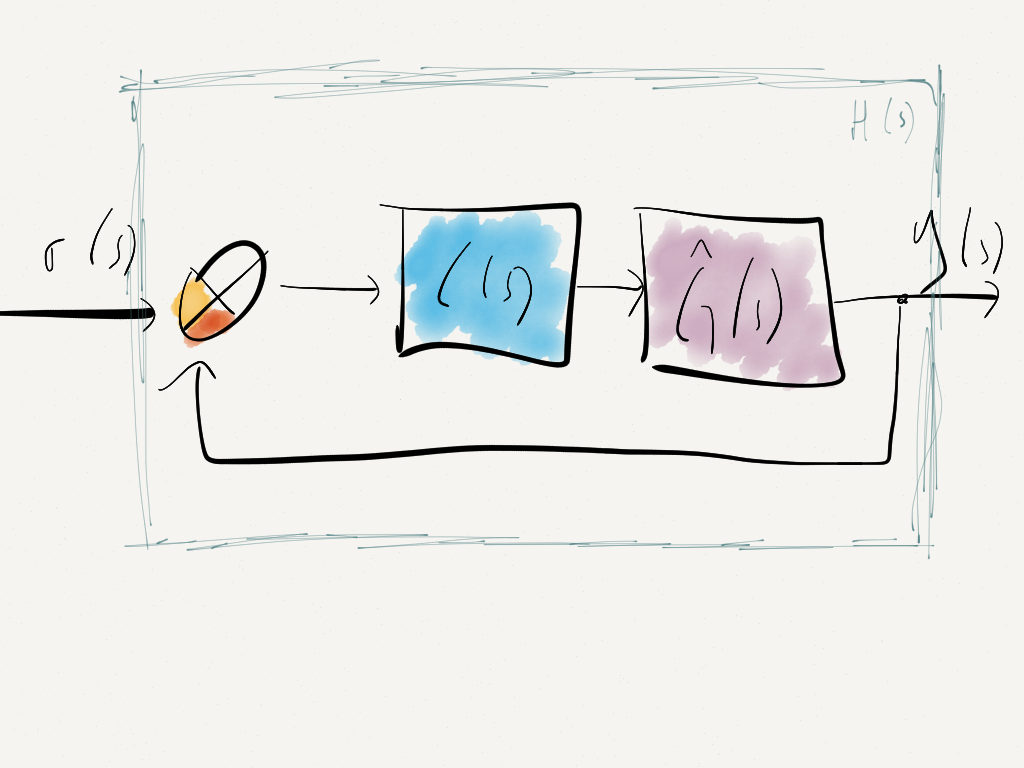
\includegraphics[width=0.4\textwidth]{../imagenes/1.png}
\end{figure*}

en donde \(\tilde{C}(s)\) será de la forma:

\begin{figure*}[h!]
\centering
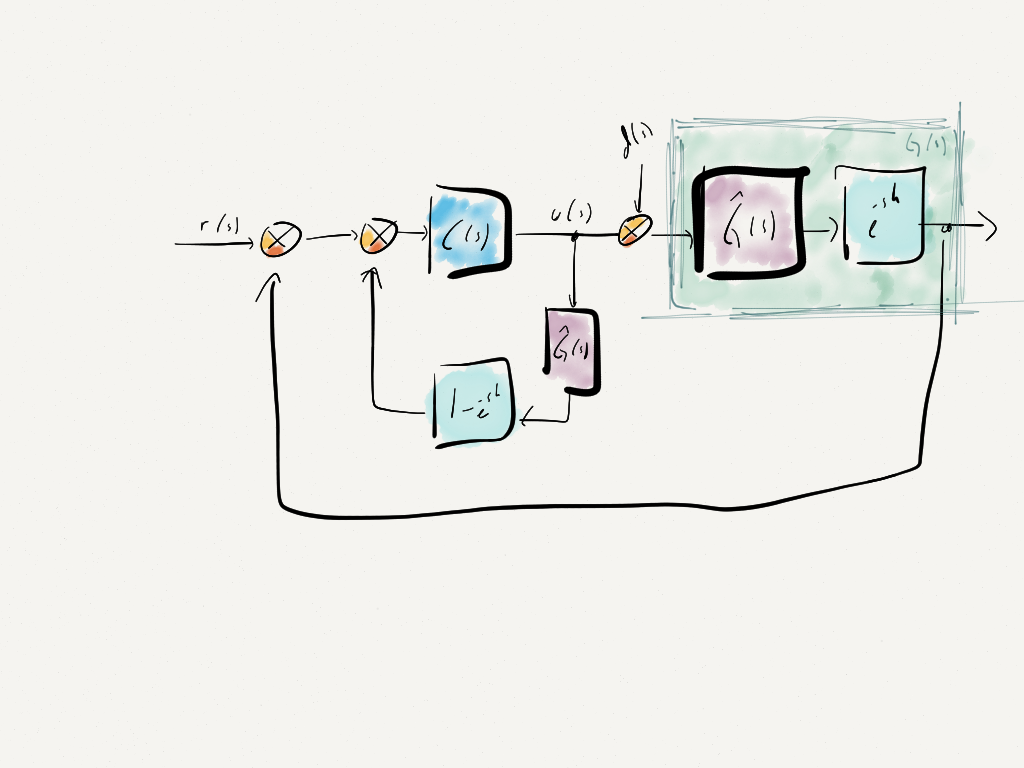
\includegraphics[width=0.4\textwidth]{../imagenes/2.png}
\end{figure*}

es decir:

\[
\tilde{C}(s) = \frac{C(s)}{1 + C(s) \hat{G}(s) \left( 1 - e^{-sh} \right)}
\]

en donde \(\hat{G}(s)\) es la parte de la función de transferencia del
sistema que no incluye al retardo. Por lo que nuestra primera tarea es
encontrar la función de transferencia para nuestro sistema sin el efecto
del retardo.

Consideremos pues el sistema

\[
\dot{x}(t) = A x(t) + B u(t)
\]

\[
y(t) = C x(t)
\]

para el cual la función de transferencia se puede obtener por la
siguiente ecuación:

\[
\hat{G}(s) = C \left( sI - A \right)^{-1} B
\]

cabe mencionar que la función de transferencia para el sistema con
retardo es:

\[
G(s) = C \left( sI - A \right)^{-1} B e^{-sh}
\]

por lo que en efecto \(\hat{G}(s)\) es la parte de la función de
transferencia del sistema sin el efecto del retardo:

\[
G(s) = \hat{G}(s) e^{-sh}
\]

    \begin{Verbatim}[commandchars=\\\{\}]
{\color{incolor}In [{\color{incolor}1}]:} \PY{c}{\PYZsh{} Se importan las librerias para calculo simbolico}
        \PY{k+kn}{from} \PY{n+nn}{IPython.display} \PY{k+kn}{import} \PY{n}{display}
        
        \PY{k+kn}{from} \PY{n+nn}{sympy} \PY{k+kn}{import} \PY{n}{var}\PY{p}{,} \PY{n}{simplify}\PY{p}{,} \PY{n}{collect}\PY{p}{,} \PY{n}{expand}\PY{p}{,} \PY{n}{solve}\PY{p}{,} \PY{n}{sin}\PY{p}{,} \PY{n}{cos}\PY{p}{,} \PY{n}{Matrix}\PY{p}{,} \PY{n}{eye}\PY{p}{,} \PY{n}{diff}\PY{p}{,} \PY{n}{Function}\PY{p}{,} \PY{n}{expand\PYZus{}power\PYZus{}base}
        \PY{k+kn}{from} \PY{n+nn}{sympy.physics.mechanics} \PY{k+kn}{import} \PY{n}{mlatex}\PY{p}{,} \PY{n}{mechanics\PYZus{}printing}
        \PY{n}{mechanics\PYZus{}printing}\PY{p}{(}\PY{p}{)}
\end{Verbatim}

    \begin{Verbatim}[commandchars=\\\{\}]
{\color{incolor}In [{\color{incolor}2}]:} \PY{o}{\PYZpc{}}\PY{k}{matplotlib} \PY{n}{inline}
        \PY{k+kn}{from} \PY{n+nn}{matplotlib.pyplot} \PY{k+kn}{import} \PY{n}{plot}\PY{p}{,} \PY{n}{style}\PY{p}{,} \PY{n}{figure}\PY{p}{,} \PY{n}{legend}
        \PY{n}{style}\PY{o}{.}\PY{n}{use}\PY{p}{(}\PY{l+s}{\PYZdq{}}\PY{l+s}{ggplot}\PY{l+s}{\PYZdq{}}\PY{p}{)}
\end{Verbatim}

    \begin{Verbatim}[commandchars=\\\{\}]
{\color{incolor}In [{\color{incolor}3}]:} \PY{k+kn}{from} \PY{n+nn}{control} \PY{k+kn}{import} \PY{n}{tf}\PY{p}{,} \PY{n}{step}\PY{p}{,} \PY{n}{pade}\PY{p}{,} \PY{n}{acker}\PY{p}{,} \PY{n}{ss}\PY{p}{,} \PY{n}{feedback}
        \PY{k+kn}{from} \PY{n+nn}{numpy} \PY{k+kn}{import} \PY{n}{linspace}\PY{p}{,} \PY{n}{matrix}\PY{p}{,} \PY{n}{eye}
\end{Verbatim}

    \begin{Verbatim}[commandchars=\\\{\}]
{\color{incolor}In [{\color{incolor}4}]:} \PY{n}{var}\PY{p}{(}\PY{l+s}{\PYZdq{}}\PY{l+s}{s}\PY{l+s}{\PYZdq{}}\PY{p}{)}
\end{Verbatim}
\texttt{\color{outcolor}Out[{\color{outcolor}4}]:}
    
    
        \begin{equation*}
        s
        \end{equation*}

    

    Empezaremos con el sistema
\(A_1 = \begin{pmatrix} 0 & 1 \\ 0 & 0 \end{pmatrix}\),
\(B_1 = \begin{pmatrix} 0 \\ 1 \end{pmatrix}\),
\(C_1 = \begin{pmatrix} 1 & 0 \end{pmatrix}\) y \(h = 1\).

    \begin{Verbatim}[commandchars=\\\{\}]
{\color{incolor}In [{\color{incolor}5}]:} \PY{n}{A1} \PY{o}{=} \PY{n}{Matrix}\PY{p}{(}\PY{p}{[}\PY{p}{[}\PY{l+m+mi}{0}\PY{p}{,} \PY{l+m+mi}{1}\PY{p}{]}\PY{p}{,} \PY{p}{[}\PY{l+m+mi}{0}\PY{p}{,} \PY{l+m+mi}{0}\PY{p}{]}\PY{p}{]}\PY{p}{)}
        \PY{n}{B1} \PY{o}{=} \PY{n}{Matrix}\PY{p}{(}\PY{p}{[}\PY{p}{[}\PY{l+m+mi}{0}\PY{p}{]}\PY{p}{,} \PY{p}{[}\PY{l+m+mi}{1}\PY{p}{]}\PY{p}{]}\PY{p}{)}
        \PY{n}{C1} \PY{o}{=} \PY{n}{Matrix}\PY{p}{(}\PY{p}{[}\PY{p}{[}\PY{l+m+mi}{1}\PY{p}{,} \PY{l+m+mi}{0}\PY{p}{]}\PY{p}{]}\PY{p}{)}
        
        \PY{n}{G1} \PY{o}{=} \PY{p}{(}\PY{n}{C1}\PY{o}{*}\PY{p}{(}\PY{n}{s}\PY{o}{*}\PY{n}{eye}\PY{p}{(}\PY{l+m+mi}{2}\PY{p}{)} \PY{o}{\PYZhy{}} \PY{n}{A1}\PY{p}{)}\PY{o}{.}\PY{n}{inv}\PY{p}{(}\PY{p}{)}\PY{o}{*}\PY{n}{B1}\PY{p}{)}\PY{p}{[}\PY{l+m+mi}{0}\PY{p}{]}
        \PY{n}{G1}
\end{Verbatim}
\texttt{\color{outcolor}Out[{\color{outcolor}5}]:}
    
    
        \begin{equation*}
        \frac{1.0}{s^{2}}
        \end{equation*}

    

    \begin{Verbatim}[commandchars=\\\{\}]
{\color{incolor}In [{\color{incolor}6}]:} \PY{n}{t} \PY{o}{=} \PY{n}{linspace}\PY{p}{(}\PY{l+m+mi}{0}\PY{p}{,} \PY{l+m+mi}{10}\PY{p}{,} \PY{l+m+mi}{100}\PY{p}{)}
        \PY{n}{t}\PY{o}{.}\PY{n}{max}\PY{p}{(}\PY{p}{)}
\end{Verbatim}
\texttt{\color{outcolor}Out[{\color{outcolor}6}]:}
    
    
        \begin{equation*}
        10.0
        \end{equation*}

    

    Podemos notar que la función de transferencia de este sistema es:

\[
G(s) = \frac{1}{s^2}
\]

    \begin{Verbatim}[commandchars=\\\{\}]
{\color{incolor}In [{\color{incolor}7}]:} \PY{c}{\PYZsh{} Convertimos las matrices simbolicas en matrices de tipo numerico}
        \PY{n}{A1} \PY{o}{=} \PY{n}{matrix}\PY{p}{(}\PY{n}{A1}\PY{o}{.}\PY{n}{tolist}\PY{p}{(}\PY{p}{)}\PY{p}{,} \PY{n}{dtype}\PY{o}{=}\PY{n+nb}{float}\PY{p}{)}
        \PY{n}{B1} \PY{o}{=} \PY{n}{matrix}\PY{p}{(}\PY{n}{B1}\PY{o}{.}\PY{n}{tolist}\PY{p}{(}\PY{p}{)}\PY{p}{,} \PY{n}{dtype}\PY{o}{=}\PY{n+nb}{float}\PY{p}{)}
        \PY{n}{C1} \PY{o}{=} \PY{n}{matrix}\PY{p}{(}\PY{n}{C1}\PY{o}{.}\PY{n}{tolist}\PY{p}{(}\PY{p}{)}\PY{p}{,} \PY{n}{dtype}\PY{o}{=}\PY{n+nb}{float}\PY{p}{)}
\end{Verbatim}

    Para obtener dos polos en \(-1\) podemos usar la función
\texttt{acker()} para obtener las ganancias de nuestro controlador PD,
el cual utilizaremos para estabilizar nuestro sistema.

    \begin{Verbatim}[commandchars=\\\{\}]
{\color{incolor}In [{\color{incolor}8}]:} \PY{n}{k1} \PY{o}{=} \PY{n}{acker}\PY{p}{(}\PY{n}{A1}\PY{p}{,} \PY{n}{B1}\PY{p}{,} \PY{p}{(}\PY{o}{\PYZhy{}}\PY{l+m+mi}{1}\PY{p}{,} \PY{o}{\PYZhy{}}\PY{l+m+mi}{1}\PY{p}{)}\PY{p}{)}
        \PY{n}{k1}
\end{Verbatim}

            \begin{Verbatim}[commandchars=\\\{\}]
{\color{outcolor}Out[{\color{outcolor}8}]:} matrix([[ 1.,  2.]])
\end{Verbatim}
        
    Definimos una función que calculará todos los controladores que
deseamos, segun la ecuación que ya dimos:

\[
\tilde{C}(s) = \frac{C(s)}{1 + C(s) \hat{G}(s) \left( 1 - e^{-sh} \right)}
\]

Al final gráfica la respuesta del sistema con y sin efecto del retardo,
asi como con y sin controlador.

    \begin{Verbatim}[commandchars=\\\{\}]
{\color{incolor}In [{\color{incolor}9}]:} \PY{k}{def} \PY{n+nf}{smith\PYZus{}predictor}\PY{p}{(}\PY{n}{A}\PY{p}{,} \PY{n}{B}\PY{p}{,} \PY{n}{C}\PY{p}{,} \PY{n}{D}\PY{p}{,} \PY{n}{k}\PY{p}{,} \PY{n}{tau}\PY{o}{=}\PY{l+m+mi}{1}\PY{p}{,} \PY{n}{t}\PY{o}{=}\PY{p}{(}\PY{l+m+mi}{0}\PY{p}{,} \PY{l+m+mi}{10}\PY{p}{)}\PY{p}{)}\PY{p}{:}
            \PY{l+s+sd}{\PYZsq{}\PYZsq{}\PYZsq{}Predictor de Smith}
        \PY{l+s+sd}{    }
        \PY{l+s+sd}{    Esta función toma los arreglos A, B, C, D de un sistema con retardo en la entrada}
        \PY{l+s+sd}{    y crea un controlador PD con los valores de k = [kp, kd] que estabiliza al sistema}
        \PY{l+s+sd}{    sin retardos. Ademas crea un controlador que estabiliza al sistema con retardo,}
        \PY{l+s+sd}{    dada la condición de que este sistema sea estable, y grafica la salida de los}
        \PY{l+s+sd}{    con y sin realimentación y con y sin retardo tau del tiempo t0 al tiempo t1}
        \PY{l+s+sd}{    especificados en t = (t0, t1).}
        \PY{l+s+sd}{    }
        \PY{l+s+sd}{    Ejemplo}
        \PY{l+s+sd}{    \PYZhy{}\PYZhy{}\PYZhy{}\PYZhy{}\PYZhy{}\PYZhy{}\PYZhy{}}
        \PY{l+s+sd}{    \PYZgt{}\PYZgt{}\PYZgt{} A1 = [[0, 1], [0, 0]]}
        \PY{l+s+sd}{    \PYZgt{}\PYZgt{}\PYZgt{} B1 = [[0], [1]]}
        \PY{l+s+sd}{    \PYZgt{}\PYZgt{}\PYZgt{} C1 = [[1, 0]]}
        \PY{l+s+sd}{    \PYZgt{}\PYZgt{}\PYZgt{} D1 = 0}
        \PY{l+s+sd}{    \PYZgt{}\PYZgt{}\PYZgt{} tau1 = 1}
        \PY{l+s+sd}{    \PYZgt{}\PYZgt{}\PYZgt{} t = (0, 10)}
        \PY{l+s+sd}{    \PYZgt{}\PYZgt{}\PYZgt{} smith\PYZus{}predictor(A1, B1, C1, D1, [1, 2], tau, t)}
        \PY{l+s+sd}{    \PYZsq{}\PYZsq{}\PYZsq{}}
            \PY{k+kn}{from} \PY{n+nn}{control} \PY{k+kn}{import} \PY{n}{ss}\PY{p}{,} \PY{n}{tf}\PY{p}{,} \PY{n}{pade}\PY{p}{,} \PY{n}{step}\PY{p}{,} \PY{n}{feedback}
            \PY{k+kn}{from} \PY{n+nn}{numpy} \PY{k+kn}{import} \PY{n}{linspace}
            \PY{k+kn}{from} \PY{n+nn}{matplotlib.pyplot} \PY{k+kn}{import} \PY{n}{figure}\PY{p}{,} \PY{n}{plot}\PY{p}{,} \PY{n}{legend}
            
            \PY{n}{kp}\PY{p}{,} \PY{n}{kd} \PY{o}{=} \PY{n}{k}
            \PY{n}{ts} \PY{o}{=} \PY{n}{linspace}\PY{p}{(}\PY{n}{t}\PY{p}{[}\PY{l+m+mi}{0}\PY{p}{]}\PY{p}{,} \PY{n}{t}\PY{p}{[}\PY{l+m+mi}{1}\PY{p}{]}\PY{p}{,} \PY{l+m+mi}{1000}\PY{p}{)}
            
            \PY{n}{sis} \PY{o}{=} \PY{n}{ss}\PY{p}{(}\PY{n}{A}\PY{p}{,} \PY{n}{B}\PY{p}{,} \PY{n}{C}\PY{p}{,} \PY{n}{D}\PY{p}{)}
            \PY{n}{cont} \PY{o}{=} \PY{n}{tf}\PY{p}{(}\PY{p}{[}\PY{n}{kd}\PY{p}{,} \PY{n}{kp}\PY{p}{]}\PY{p}{,} \PY{p}{[}\PY{l+m+mi}{0}\PY{p}{,} \PY{l+m+mi}{1}\PY{p}{]}\PY{p}{)}
            
            \PY{n}{num}\PY{p}{,} \PY{n}{den} \PY{o}{=} \PY{n}{pade}\PY{p}{(}\PY{n}{T}\PY{o}{=}\PY{n}{tau}\PY{p}{,} \PY{n}{n}\PY{o}{=}\PY{l+m+mi}{10}\PY{p}{)}
            \PY{n}{delay} \PY{o}{=} \PY{n}{tf}\PY{p}{(}\PY{n}{num}\PY{p}{,} \PY{n}{den}\PY{p}{)}
            
            \PY{n}{delcont} \PY{o}{=} \PY{p}{(}\PY{p}{(}\PY{l+m+mi}{1} \PY{o}{\PYZhy{}} \PY{n}{delay}\PY{p}{)}\PY{o}{*}\PY{n}{sis}\PY{p}{)}
            
            \PY{n}{y}\PY{p}{,} \PY{n}{t1} \PY{o}{=} \PY{n}{step}\PY{p}{(}\PY{n}{sis}\PY{p}{,} \PY{n}{ts}\PY{p}{)}
            \PY{n}{yd}\PY{p}{,} \PY{n}{td} \PY{o}{=} \PY{n}{step}\PY{p}{(}\PY{n}{sis}\PY{o}{*}\PY{n}{delay}\PY{p}{,} \PY{n}{ts}\PY{p}{)}
            \PY{n}{ycont}\PY{p}{,} \PY{n}{tcont} \PY{o}{=} \PY{n}{step}\PY{p}{(}\PY{p}{(}\PY{n}{cont}\PY{o}{*}\PY{n}{sis}\PY{p}{)}\PY{o}{.}\PY{n}{feedback}\PY{p}{(}\PY{p}{)}\PY{p}{,} \PY{n}{ts}\PY{p}{)}
            \PY{n}{ycontdel}\PY{p}{,} \PY{n}{tcontdel} \PY{o}{=} \PY{n}{step}\PY{p}{(}\PY{n}{feedback}\PY{p}{(}\PY{n}{feedback}\PY{p}{(}\PY{n}{cont}\PY{p}{,} \PY{n}{delcont}\PY{p}{)}\PY{o}{*}\PY{n}{sis}\PY{p}{)}\PY{p}{,} \PY{n}{ts}\PY{p}{)}
            
            \PY{n}{f} \PY{o}{=} \PY{n}{figure}\PY{p}{(}\PY{n}{figsize}\PY{o}{=}\PY{p}{(}\PY{l+m+mi}{10}\PY{p}{,} \PY{l+m+mi}{6}\PY{p}{)}\PY{p}{)}
        
            \PY{n}{p1}\PY{p}{,} \PY{o}{=} \PY{n}{plot}\PY{p}{(}\PY{n}{td}\PY{p}{,} \PY{n}{yd}\PY{p}{)}
            \PY{n}{p2}\PY{p}{,} \PY{o}{=} \PY{n}{plot}\PY{p}{(}\PY{n}{t1}\PY{p}{,} \PY{n}{y}\PY{p}{)}
            \PY{n}{p3}\PY{p}{,} \PY{o}{=} \PY{n}{plot}\PY{p}{(}\PY{n}{tcont}\PY{p}{,} \PY{n}{ycont}\PY{p}{)}
            \PY{n}{p4}\PY{p}{,} \PY{o}{=} \PY{n}{plot}\PY{p}{(}\PY{n}{tcontdel}\PY{p}{,} \PY{n}{ycontdel}\PY{p}{)}
        
            \PY{n}{ax} \PY{o}{=} \PY{n}{f}\PY{o}{.}\PY{n}{gca}\PY{p}{(}\PY{p}{)}
            \PY{n}{ax}\PY{o}{.}\PY{n}{set\PYZus{}xlim}\PY{p}{(}\PY{n}{t}\PY{p}{[}\PY{l+m+mi}{0}\PY{p}{]} \PY{o}{\PYZhy{}} \PY{l+m+mf}{0.1}\PY{p}{,} \PY{n}{t}\PY{p}{[}\PY{l+m+mi}{1}\PY{p}{]}\PY{p}{)}
            \PY{n}{ax}\PY{o}{.}\PY{n}{set\PYZus{}ylim}\PY{p}{(}\PY{o}{\PYZhy{}}\PY{l+m+mf}{0.10}\PY{o}{*}\PY{n}{ycont}\PY{o}{.}\PY{n}{max}\PY{p}{(}\PY{p}{)}\PY{p}{,} \PY{l+m+mf}{1.1}\PY{o}{*}\PY{n}{ycont}\PY{o}{.}\PY{n}{max}\PY{p}{(}\PY{p}{)}\PY{p}{)}
        
            \PY{n}{ax}\PY{o}{.}\PY{n}{set\PYZus{}ylabel}\PY{p}{(}\PY{l+s}{r\PYZdq{}}\PY{l+s}{\PYZdl{}y(t)\PYZdl{}}\PY{l+s}{\PYZdq{}}\PY{p}{,} \PY{n}{fontsize}\PY{o}{=}\PY{l+m+mi}{20}\PY{p}{)}
            \PY{n}{ax}\PY{o}{.}\PY{n}{set\PYZus{}xlabel}\PY{p}{(}\PY{l+s}{r\PYZdq{}}\PY{l+s}{\PYZdl{}t\PYZdl{}}\PY{l+s}{\PYZdq{}}\PY{p}{,} \PY{n}{fontsize}\PY{o}{=}\PY{l+m+mi}{20}\PY{p}{)}
        
            \PY{n}{legend}\PY{p}{(}\PY{p}{[}\PY{n}{p1}\PY{p}{,} \PY{n}{p2}\PY{p}{,} \PY{n}{p3}\PY{p}{,} \PY{n}{p4}\PY{p}{]}\PY{p}{,}
                   \PY{p}{[}\PY{l+s}{r\PYZdq{}}\PY{l+s}{\PYZdl{}G(s)\PYZdl{}}\PY{l+s}{\PYZdq{}}\PY{p}{,}
                    \PY{l+s}{r\PYZdq{}}\PY{l+s}{\PYZdl{}}\PY{l+s}{\PYZbs{}}\PY{l+s}{hat\PYZob{}G\PYZcb{}(s)\PYZdl{}}\PY{l+s}{\PYZdq{}}\PY{p}{,}
                    \PY{l+s}{r\PYZdq{}}\PY{l+s}{\PYZdl{}}\PY{l+s}{\PYZbs{}}\PY{l+s}{hat\PYZob{}G\PYZcb{}\PYZus{}F(s)\PYZdl{}}\PY{l+s}{\PYZdq{}}\PY{p}{,}
                    \PY{l+s}{r\PYZdq{}}\PY{l+s}{\PYZdl{}G\PYZus{}F(s)\PYZdl{}}\PY{l+s}{\PYZdq{}}\PY{p}{]}\PY{p}{,} \PY{n}{loc}\PY{o}{=}\PY{l+m+mi}{4}\PY{p}{,} \PY{n}{fontsize}\PY{o}{=}\PY{l+m+mi}{16}\PY{p}{)}\PY{p}{;}
\end{Verbatim}

    Por lo que si le damos nuestro sistema con las ganancias deseadas, asi
como el tiempo para el que nos interesa, y el retardo, tendremos:

    \begin{Verbatim}[commandchars=\\\{\}]
{\color{incolor}In [{\color{incolor}17}]:} \PY{n}{smith\PYZus{}predictor}\PY{p}{(}\PY{n}{A1}\PY{p}{,} \PY{n}{B1}\PY{p}{,} \PY{n}{C1}\PY{p}{,} \PY{l+m+mi}{0}\PY{p}{,} \PY{n}{k}\PY{o}{=}\PY{p}{[}\PY{l+m+mi}{3}\PY{p}{,} \PY{l+m+mi}{3}\PY{p}{]}\PY{p}{,} \PY{n}{t}\PY{o}{=}\PY{p}{(}\PY{l+m+mi}{0}\PY{p}{,} \PY{l+m+mi}{7}\PY{p}{)}\PY{p}{,} \PY{n}{tau}\PY{o}{=}\PY{l+m+mi}{1}\PY{p}{)}
\end{Verbatim}

    \begin{center}
    \adjustimage{max size={0.9\linewidth}{0.9\paperheight}}{Tarea 8_files/Tarea 8_19_0.png}
    \end{center}
    { \hspace*{\fill} \\}
    
    Ahora definimos el sistema
\(A_2 = \begin{pmatrix} 0 & 1 \\ -1 & 0 \end{pmatrix}\),
\(B_2 = \begin{pmatrix} 0 \\ 1 \end{pmatrix}\),
\(C_2 = \begin{pmatrix} 1 & 0 \end{pmatrix}\) y \(h = 1\).

    \begin{Verbatim}[commandchars=\\\{\}]
{\color{incolor}In [{\color{incolor}11}]:} \PY{n}{A2} \PY{o}{=} \PY{n}{Matrix}\PY{p}{(}\PY{p}{[}\PY{p}{[}\PY{l+m+mi}{0}\PY{p}{,} \PY{l+m+mi}{1}\PY{p}{]}\PY{p}{,} \PY{p}{[}\PY{o}{\PYZhy{}}\PY{l+m+mi}{1}\PY{p}{,} \PY{l+m+mi}{0}\PY{p}{]}\PY{p}{]}\PY{p}{)}
         \PY{n}{B2} \PY{o}{=} \PY{n}{Matrix}\PY{p}{(}\PY{p}{[}\PY{p}{[}\PY{l+m+mi}{0}\PY{p}{]}\PY{p}{,} \PY{p}{[}\PY{l+m+mi}{1}\PY{p}{]}\PY{p}{]}\PY{p}{)}
         \PY{n}{C2} \PY{o}{=} \PY{n}{Matrix}\PY{p}{(}\PY{p}{[}\PY{p}{[}\PY{l+m+mi}{1}\PY{p}{,} \PY{l+m+mi}{0}\PY{p}{]}\PY{p}{]}\PY{p}{)}
         
         \PY{n}{G2} \PY{o}{=} \PY{p}{(}\PY{n}{C2}\PY{o}{*}\PY{p}{(}\PY{n}{s}\PY{o}{*}\PY{n}{eye}\PY{p}{(}\PY{l+m+mi}{2}\PY{p}{)} \PY{o}{\PYZhy{}} \PY{n}{A2}\PY{p}{)}\PY{o}{.}\PY{n}{inv}\PY{p}{(}\PY{p}{)}\PY{o}{*}\PY{n}{B2}\PY{p}{)}\PY{p}{[}\PY{l+m+mi}{0}\PY{p}{]}
         \PY{n}{G2}
\end{Verbatim}
\texttt{\color{outcolor}Out[{\color{outcolor}11}]:}
    
    
        \begin{equation*}
        \frac{1.0}{s \left(1.0 s + \frac{1.0}{s}\right)}
        \end{equation*}

    

    Por lo que la función de transferencia de este sistema es:

\[
G(s) = \frac{1}{s^2 + 1}
\]

    \begin{Verbatim}[commandchars=\\\{\}]
{\color{incolor}In [{\color{incolor}12}]:} \PY{c}{\PYZsh{} Convertimos las matrices simbolicas en matrices de tipo numerico}
         \PY{n}{A2} \PY{o}{=} \PY{n}{matrix}\PY{p}{(}\PY{n}{A2}\PY{o}{.}\PY{n}{tolist}\PY{p}{(}\PY{p}{)}\PY{p}{,} \PY{n}{dtype}\PY{o}{=}\PY{n+nb}{float}\PY{p}{)}
         \PY{n}{B2} \PY{o}{=} \PY{n}{matrix}\PY{p}{(}\PY{n}{B2}\PY{o}{.}\PY{n}{tolist}\PY{p}{(}\PY{p}{)}\PY{p}{,} \PY{n}{dtype}\PY{o}{=}\PY{n+nb}{float}\PY{p}{)}
         \PY{n}{C2} \PY{o}{=} \PY{n}{matrix}\PY{p}{(}\PY{n}{C2}\PY{o}{.}\PY{n}{tolist}\PY{p}{(}\PY{p}{)}\PY{p}{,} \PY{n}{dtype}\PY{o}{=}\PY{n+nb}{float}\PY{p}{)}
\end{Verbatim}

    Para obtener dos polos en \(-1\) podemos usar la función
\texttt{acker()} para obtener las ganancias de nuestro controlador PD.

    \begin{Verbatim}[commandchars=\\\{\}]
{\color{incolor}In [{\color{incolor}13}]:} \PY{n}{k2} \PY{o}{=} \PY{n}{acker}\PY{p}{(}\PY{n}{A2}\PY{p}{,} \PY{n}{B2}\PY{p}{,} \PY{p}{(}\PY{o}{\PYZhy{}}\PY{l+m+mi}{1}\PY{p}{,} \PY{o}{\PYZhy{}}\PY{l+m+mi}{1}\PY{p}{)}\PY{p}{)}
         \PY{n}{k2}
\end{Verbatim}

            \begin{Verbatim}[commandchars=\\\{\}]
{\color{outcolor}Out[{\color{outcolor}13}]:} matrix([[ 0.,  2.]])
\end{Verbatim}
        
    Y la respuesta del sistema es:

    \begin{Verbatim}[commandchars=\\\{\}]
{\color{incolor}In [{\color{incolor}18}]:} \PY{n}{smith\PYZus{}predictor}\PY{p}{(}\PY{n}{A2}\PY{p}{,} \PY{n}{B2}\PY{p}{,} \PY{n}{C2}\PY{p}{,} \PY{l+m+mi}{0}\PY{p}{,} \PY{n}{k}\PY{o}{=}\PY{p}{[}\PY{l+m+mi}{3}\PY{p}{,} \PY{l+m+mi}{3}\PY{p}{]}\PY{p}{,} \PY{n}{t}\PY{o}{=}\PY{p}{(}\PY{l+m+mi}{0}\PY{p}{,} \PY{l+m+mi}{8}\PY{p}{)}\PY{p}{)}
\end{Verbatim}

    \begin{center}
    \adjustimage{max size={0.9\linewidth}{0.9\paperheight}}{Tarea 8_files/Tarea 8_27_0.png}
    \end{center}
    { \hspace*{\fill} \\}
    
    Puedes acceder a este notebook a traves de la página

http://bit.ly/1wiwlpl

o escaneando el siguiente código:

\begin{figure*}[htbp]
\centering

\includegraphics[width=0.2\textwidth]{../codigos/codigo8.jpg}
\end{figure*}
        

    % Add a bibliography block to the postdoc
    
    
    
    \end{document}
